\chapter{Supersymmetry and MSSM}
We have already seen the the standard model 
performs fantastically well in describing experimental observations. The
recent discovery of a standard model-like higgs boson brings with it
more confidence of the model. 
As seen in the previous chapter, the potential of the standard model higgs 
field is,
\begin{equation}
V=m_{h}^{2}(\phi)+\lambda(\phi)^{2}
\end{equation}
where $\phi$ is a complex scalar.
A non vanishing vacuum expectation 
value of $246 \GeV$ is required for spontaneous symmetry breaking.
However, a problem arises when 
considering higher order loop corrections to the mass of the higgs as shown in
figure \ref{fig:fermionLoop} 
If a fermion couples to the higgs with a term in the Lagrangian $-\lambda_{f}\phi \bar{f}f$
then figure \ref{fig:fermionLoop} 
yields a correction the the higgs mass,
\begin{equation}
\Delta m_{H}^{2}=-\frac{|\lambda_{f}|^{2}}{8\pi^{2}}\Lambda_{UV}^{2}+...
\label{eq:SUS1}
\end{equation}
where $\Lambda_{UV}$ is an ultraviolet cutoff to regulate the loop. $\Lambda_{UV}$
is also the energy scale at which new physics should enter.
Accordingly, we have quantum corrections from the virtual 
effects of every particle that couples to the higgs. Furthermore if each of these 
particles gain their mass through the higgs mechanism the entire standard model 
mass spectrum is sensitive to the ultraviolet cutoff.
%Since the electroweak gauge bosons, and possibly the quarks and leptons gain their
%mass from the Higgs Mechanism 
However, suppose there exists a massive scalar particle S, mass $m_{S}$, that couples
to the higgs with a term $-\lambda_{S}\phi^{2} S^{2}$
figure \ref{fig:scalarLoop} would give a correction of,
\begin{equation}
\Delta m_{H}^{2}=\frac{\lambda_{s}}{16\pi^{2}}\left[\Lambda_{UV}^{2}-2m_{s}^{2}ln(\Lambda_{UV}/m_{S})+... \right].
\label{eq:SUS2}
\end{equation}
By examining (\ref{eq:SUS1}) and the second term of (\ref{eq:SUS2}) it is apparent that if each of the quarks
and leptons is accompanied by 2 complex scalars the $\Lambda_{UV}^{2}$ terms will cancel.
%This problem is known as the Hierarchy Problem. %%cite

\begin{figure}[hb]
  \centering
  \begin{subfigure}[trim = 0mm 0mm 0mm 0mm, clip, width=3cm]{.4\textwidth}
	\marginbox{0mm 0pt 0mm 0pt}{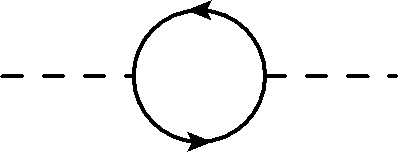
\includegraphics[width=\textwidth]{images/fermionLoop.png}}
                %\marginbox{-10mm 0pt 10mm 0pt}{
                \caption{}
                \label{fig:fermionLoop}
\end{subfigure}
\begin{subfigure}[trim = 0mm 0mm 0mm 0mm, clip, width=3cm]{.4\textwidth}
	\marginbox{0mm 0pt 0mm 0pt}{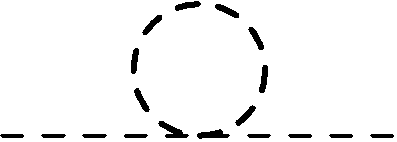
\includegraphics[width=\textwidth]{images/SLoop.png}}
	\caption{}
                %\marginbox{10mm 0pt -10mm 0pt}{}
                \label{fig:scalarLoop}
                	
  \end{subfigure}
   \caption[]{One loop quantum corrections for a fermion (\ref{fig:scalarLoop}) and a scalar (\ref{fig:scalarLoop}). }
\end{figure}

A supersymmetry transformation changes a fermionic state into a bosonic state and vice versa,
\begin{equation}
Q|Boson\rangle=|Fermion\rangle \qquad Q|Fermion\rangle=|Boson\rangle
\end{equation}

\begin{equation}
\{Q,Q^{\dagger}\}=p^{\mu}
\end{equation}
\begin{equation}
\{Q,Q\}=\{Q^{\dagger},Q^{\dagger}\}=0
\end{equation}
\begin{equation}
[p^{\mu},Q ]=[p^{\mu},Q^{\dagger}]=0
\end{equation}

\section{MSSM Higgs Production}